% Created by tikzDevice version 0.12.3.1 on 2021-07-06 19:35:49
% !TEX encoding = UTF-8 Unicode
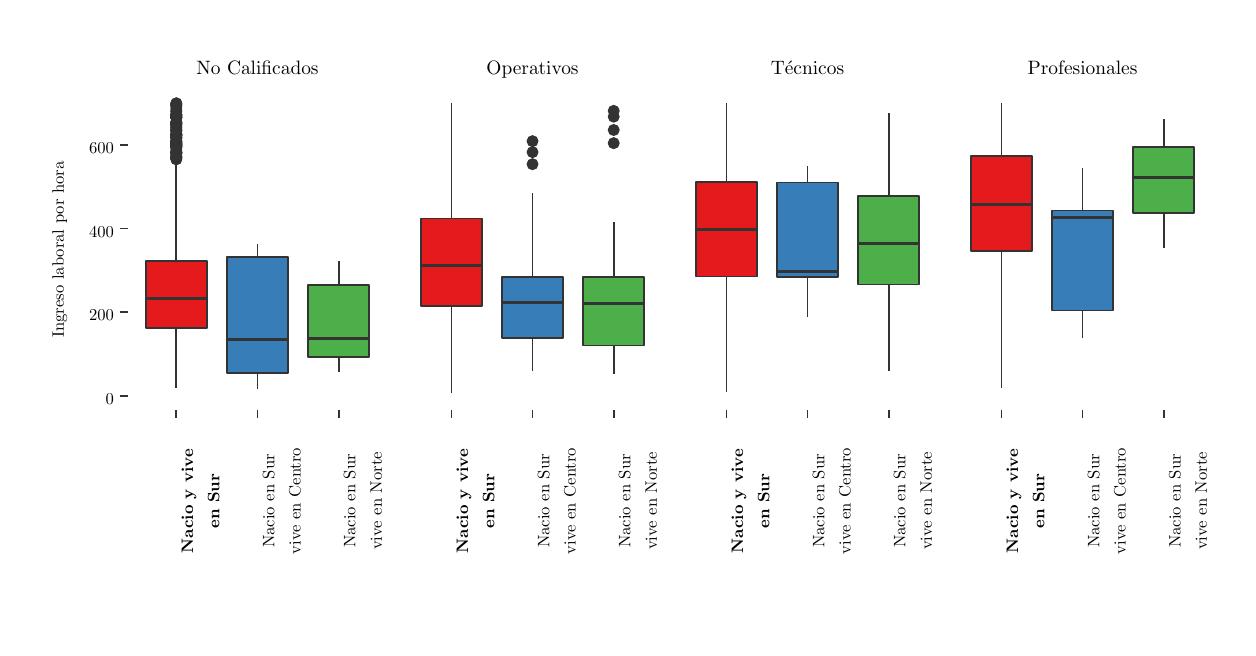
\begin{tikzpicture}[x=1pt,y=1pt]
\definecolor{fillColor}{RGB}{255,255,255}
\path[use as bounding box,fill=fillColor,fill opacity=0.00] (0,0) rectangle (433.62,216.81);
\begin{scope}
\path[clip] (  0.00,  0.00) rectangle (433.62,216.81);
\definecolor{drawColor}{RGB}{255,255,255}
\definecolor{fillColor}{RGB}{255,255,255}

\path[draw=drawColor,line width= 0.6pt,line join=round,line cap=round,fill=fillColor] (  0.00,  0.00) rectangle (433.62,216.81);
\end{scope}
\begin{scope}
\path[clip] ( 36.11, 78.54) rectangle (129.99,194.74);
\definecolor{drawColor}{RGB}{255,255,255}

\path[draw=drawColor,line width= 0.3pt,line join=round] ( 36.11, 98.91) --
	(129.99, 98.91);

\path[draw=drawColor,line width= 0.3pt,line join=round] ( 36.11,129.09) --
	(129.99,129.09);

\path[draw=drawColor,line width= 0.3pt,line join=round] ( 36.11,159.27) --
	(129.99,159.27);

\path[draw=drawColor,line width= 0.3pt,line join=round] ( 36.11,189.46) --
	(129.99,189.46);

\path[draw=drawColor,line width= 0.6pt,line join=round] ( 36.11, 83.82) --
	(129.99, 83.82);

\path[draw=drawColor,line width= 0.6pt,line join=round] ( 36.11,114.00) --
	(129.99,114.00);

\path[draw=drawColor,line width= 0.6pt,line join=round] ( 36.11,144.18) --
	(129.99,144.18);

\path[draw=drawColor,line width= 0.6pt,line join=round] ( 36.11,174.37) --
	(129.99,174.37);

\path[draw=drawColor,line width= 0.6pt,line join=round] ( 53.71, 78.54) --
	( 53.71,194.74);

\path[draw=drawColor,line width= 0.6pt,line join=round] ( 83.05, 78.54) --
	( 83.05,194.74);

\path[draw=drawColor,line width= 0.6pt,line join=round] (112.39, 78.54) --
	(112.39,194.74);
\definecolor{drawColor}{gray}{0.20}
\definecolor{fillColor}{gray}{0.20}

\path[draw=drawColor,line width= 0.4pt,line join=round,line cap=round,fill=fillColor] ( 53.71,175.69) circle (  1.96);

\path[draw=drawColor,line width= 0.4pt,line join=round,line cap=round,fill=fillColor] ( 53.71,179.73) circle (  1.96);

\path[draw=drawColor,line width= 0.4pt,line join=round,line cap=round,fill=fillColor] ( 53.71,175.69) circle (  1.96);

\path[draw=drawColor,line width= 0.4pt,line join=round,line cap=round,fill=fillColor] ( 53.71,180.28) circle (  1.96);

\path[draw=drawColor,line width= 0.4pt,line join=round,line cap=round,fill=fillColor] ( 53.71,177.77) circle (  1.96);

\path[draw=drawColor,line width= 0.4pt,line join=round,line cap=round,fill=fillColor] ( 53.71,188.21) circle (  1.96);

\path[draw=drawColor,line width= 0.4pt,line join=round,line cap=round,fill=fillColor] ( 53.71,185.23) circle (  1.96);

\path[draw=drawColor,line width= 0.4pt,line join=round,line cap=round,fill=fillColor] ( 53.71,171.51) circle (  1.96);

\path[draw=drawColor,line width= 0.4pt,line join=round,line cap=round,fill=fillColor] ( 53.71,170.05) circle (  1.96);

\path[draw=drawColor,line width= 0.4pt,line join=round,line cap=round,fill=fillColor] ( 53.71,170.05) circle (  1.96);

\path[draw=drawColor,line width= 0.4pt,line join=round,line cap=round,fill=fillColor] ( 53.71,170.05) circle (  1.96);

\path[draw=drawColor,line width= 0.4pt,line join=round,line cap=round,fill=fillColor] ( 53.71,175.80) circle (  1.96);

\path[draw=drawColor,line width= 0.4pt,line join=round,line cap=round,fill=fillColor] ( 53.71,178.12) circle (  1.96);

\path[draw=drawColor,line width= 0.4pt,line join=round,line cap=round,fill=fillColor] ( 53.71,170.46) circle (  1.96);

\path[draw=drawColor,line width= 0.4pt,line join=round,line cap=round,fill=fillColor] ( 53.71,169.49) circle (  1.96);

\path[draw=drawColor,line width= 0.4pt,line join=round,line cap=round,fill=fillColor] ( 53.71,169.49) circle (  1.96);

\path[draw=drawColor,line width= 0.4pt,line join=round,line cap=round,fill=fillColor] ( 53.71,181.85) circle (  1.96);

\path[draw=drawColor,line width= 0.4pt,line join=round,line cap=round,fill=fillColor] ( 53.71,181.85) circle (  1.96);

\path[draw=drawColor,line width= 0.4pt,line join=round,line cap=round,fill=fillColor] ( 53.71,181.85) circle (  1.96);

\path[draw=drawColor,line width= 0.4pt,line join=round,line cap=round,fill=fillColor] ( 53.71,173.45) circle (  1.96);

\path[draw=drawColor,line width= 0.4pt,line join=round,line cap=round,fill=fillColor] ( 53.71,175.32) circle (  1.96);

\path[draw=drawColor,line width= 0.4pt,line join=round,line cap=round,fill=fillColor] ( 53.71,176.95) circle (  1.96);

\path[draw=drawColor,line width= 0.4pt,line join=round,line cap=round,fill=fillColor] ( 53.71,176.95) circle (  1.96);

\path[draw=drawColor,line width= 0.4pt,line join=round,line cap=round,fill=fillColor] ( 53.71,174.01) circle (  1.96);

\path[draw=drawColor,line width= 0.4pt,line join=round,line cap=round,fill=fillColor] ( 53.71,179.83) circle (  1.96);

\path[draw=drawColor,line width= 0.4pt,line join=round,line cap=round,fill=fillColor] ( 53.71,177.87) circle (  1.96);

\path[draw=drawColor,line width= 0.4pt,line join=round,line cap=round,fill=fillColor] ( 53.71,174.74) circle (  1.96);

\path[draw=drawColor,line width= 0.4pt,line join=round,line cap=round,fill=fillColor] ( 53.71,171.60) circle (  1.96);

\path[draw=drawColor,line width= 0.4pt,line join=round,line cap=round,fill=fillColor] ( 53.71,175.26) circle (  1.96);

\path[draw=drawColor,line width= 0.4pt,line join=round,line cap=round,fill=fillColor] ( 53.71,182.48) circle (  1.96);

\path[draw=drawColor,line width= 0.4pt,line join=round,line cap=round,fill=fillColor] ( 53.71,185.30) circle (  1.96);

\path[draw=drawColor,line width= 0.4pt,line join=round,line cap=round,fill=fillColor] ( 53.71,185.30) circle (  1.96);

\path[draw=drawColor,line width= 0.4pt,line join=round,line cap=round,fill=fillColor] ( 53.71,185.30) circle (  1.96);

\path[draw=drawColor,line width= 0.4pt,line join=round,line cap=round,fill=fillColor] ( 53.71,182.48) circle (  1.96);

\path[draw=drawColor,line width= 0.4pt,line join=round,line cap=round,fill=fillColor] ( 53.71,178.53) circle (  1.96);

\path[draw=drawColor,line width= 0.4pt,line join=round,line cap=round,fill=fillColor] ( 53.71,182.48) circle (  1.96);

\path[draw=drawColor,line width= 0.4pt,line join=round,line cap=round,fill=fillColor] ( 53.71,172.61) circle (  1.96);

\path[draw=drawColor,line width= 0.4pt,line join=round,line cap=round,fill=fillColor] ( 53.71,173.68) circle (  1.96);

\path[draw=drawColor,line width= 0.4pt,line join=round,line cap=round,fill=fillColor] ( 53.71,184.46) circle (  1.96);

\path[draw=drawColor,line width= 0.4pt,line join=round,line cap=round,fill=fillColor] ( 53.71,184.46) circle (  1.96);

\path[draw=drawColor,line width= 0.4pt,line join=round,line cap=round,fill=fillColor] ( 53.71,180.87) circle (  1.96);

\path[draw=drawColor,line width= 0.4pt,line join=round,line cap=round,fill=fillColor] ( 53.71,177.27) circle (  1.96);

\path[draw=drawColor,line width= 0.4pt,line join=round,line cap=round,fill=fillColor] ( 53.71,173.68) circle (  1.96);

\path[draw=drawColor,line width= 0.4pt,line join=round,line cap=round,fill=fillColor] ( 53.71,188.65) circle (  1.96);

\path[draw=drawColor,line width= 0.4pt,line join=round,line cap=round,fill=fillColor] ( 53.71,171.50) circle (  1.96);

\path[draw=drawColor,line width= 0.4pt,line join=round,line cap=round,fill=fillColor] ( 53.71,176.98) circle (  1.96);

\path[draw=drawColor,line width= 0.4pt,line join=round,line cap=round,fill=fillColor] ( 53.71,189.04) circle (  1.96);

\path[draw=drawColor,line width= 0.4pt,line join=round,line cap=round,fill=fillColor] ( 53.71,171.50) circle (  1.96);

\path[draw=drawColor,line width= 0.4pt,line join=round,line cap=round,fill=fillColor] ( 53.71,169.22) circle (  1.96);

\path[draw=drawColor,line width= 0.4pt,line join=round,line cap=round,fill=fillColor] ( 53.71,175.88) circle (  1.96);

\path[draw=drawColor,line width= 0.4pt,line join=round,line cap=round,fill=fillColor] ( 53.71,185.28) circle (  1.96);

\path[draw=drawColor,line width= 0.4pt,line join=round,line cap=round,fill=fillColor] ( 53.71,177.76) circle (  1.96);

\path[draw=drawColor,line width= 0.4pt,line join=round,line cap=round,fill=fillColor] ( 53.71,185.28) circle (  1.96);

\path[draw=drawColor,line width= 0.4pt,line join=round,line cap=round,fill=fillColor] ( 53.71,189.04) circle (  1.96);

\path[draw=drawColor,line width= 0.4pt,line join=round,line cap=round,fill=fillColor] ( 53.71,173.78) circle (  1.96);

\path[draw=drawColor,line width= 0.4pt,line join=round,line cap=round,fill=fillColor] ( 53.71,182.38) circle (  1.96);

\path[draw=drawColor,line width= 0.4pt,line join=round,line cap=round,fill=fillColor] ( 53.71,175.08) circle (  1.96);

\path[draw=drawColor,line width= 0.4pt,line join=round,line cap=round,fill=fillColor] ( 53.71,179.64) circle (  1.96);

\path[draw=drawColor,line width= 0.4pt,line join=round,line cap=round,fill=fillColor] ( 53.71,181.60) circle (  1.96);

\path[draw=drawColor,line width= 0.4pt,line join=round,line cap=round,fill=fillColor] ( 53.71,175.08) circle (  1.96);

\path[draw=drawColor,line width= 0.4pt,line join=round,line cap=round,fill=fillColor] ( 53.71,184.21) circle (  1.96);

\path[draw=drawColor,line width= 0.4pt,line join=round,line cap=round,fill=fillColor] ( 53.71,186.49) circle (  1.96);

\path[draw=drawColor,line width= 0.4pt,line join=round,line cap=round,fill=fillColor] ( 53.71,186.49) circle (  1.96);

\path[draw=drawColor,line width= 0.4pt,line join=round,line cap=round,fill=fillColor] ( 53.71,175.08) circle (  1.96);

\path[draw=drawColor,line width= 0.4pt,line join=round,line cap=round,fill=fillColor] ( 53.71,182.69) circle (  1.96);

\path[draw=drawColor,line width= 0.4pt,line join=round,line cap=round,fill=fillColor] ( 53.71,180.83) circle (  1.96);

\path[draw=drawColor,line width= 0.4pt,line join=round,line cap=round,fill=fillColor] ( 53.71,182.04) circle (  1.96);

\path[draw=drawColor,line width= 0.4pt,line join=round,line cap=round,fill=fillColor] ( 53.71,174.77) circle (  1.96);

\path[draw=drawColor,line width= 0.4pt,line join=round,line cap=round,fill=fillColor] ( 53.71,179.31) circle (  1.96);

\path[draw=drawColor,line width= 0.4pt,line join=round,line cap=round,fill=fillColor] ( 53.71,171.13) circle (  1.96);

\path[draw=drawColor,line width= 0.4pt,line join=round,line cap=round,fill=fillColor] ( 53.71,187.30) circle (  1.96);

\path[draw=drawColor,line width= 0.4pt,line join=round,line cap=round,fill=fillColor] ( 53.71,174.37) circle (  1.96);

\path[draw=drawColor,line width= 0.4pt,line join=round,line cap=round,fill=fillColor] ( 53.71,171.85) circle (  1.96);

\path[draw=drawColor,line width= 0.4pt,line join=round,line cap=round,fill=fillColor] ( 53.71,178.14) circle (  1.96);

\path[draw=drawColor,line width= 0.4pt,line join=round,line cap=round,fill=fillColor] ( 53.71,178.14) circle (  1.96);

\path[draw=drawColor,line width= 0.4pt,line join=round,line cap=round,fill=fillColor] ( 53.71,184.43) circle (  1.96);

\path[draw=drawColor,line width= 0.4pt,line join=round,line cap=round,fill=fillColor] ( 53.71,184.43) circle (  1.96);

\path[draw=drawColor,line width= 0.4pt,line join=round,line cap=round,fill=fillColor] ( 53.71,174.37) circle (  1.96);

\path[draw=drawColor,line width= 0.4pt,line join=round,line cap=round,fill=fillColor] ( 53.71,178.14) circle (  1.96);

\path[draw=drawColor,line width= 0.4pt,line join=round,line cap=round,fill=fillColor] ( 53.71,171.85) circle (  1.96);

\path[draw=drawColor,line width= 0.4pt,line join=round,line cap=round,fill=fillColor] ( 53.71,171.85) circle (  1.96);

\path[draw=drawColor,line width= 0.4pt,line join=round,line cap=round,fill=fillColor] ( 53.71,178.14) circle (  1.96);

\path[draw=drawColor,line width= 0.4pt,line join=round,line cap=round,fill=fillColor] ( 53.71,174.37) circle (  1.96);

\path[draw=drawColor,line width= 0.4pt,line join=round,line cap=round,fill=fillColor] ( 53.71,170.05) circle (  1.96);

\path[draw=drawColor,line width= 0.4pt,line join=round,line cap=round,fill=fillColor] ( 53.71,184.43) circle (  1.96);

\path[draw=drawColor,line width= 0.4pt,line join=round,line cap=round,fill=fillColor] ( 53.71,184.43) circle (  1.96);

\path[draw=drawColor,line width= 0.4pt,line join=round,line cap=round,fill=fillColor] ( 53.71,178.14) circle (  1.96);

\path[draw=drawColor,line width= 0.4pt,line join=round,line cap=round,fill=fillColor] ( 53.71,174.37) circle (  1.96);

\path[draw=drawColor,line width= 0.4pt,line join=round,line cap=round,fill=fillColor] ( 53.71,189.46) circle (  1.96);

\path[draw=drawColor,line width= 0.4pt,line join=round,line cap=round,fill=fillColor] ( 53.71,189.46) circle (  1.96);

\path[draw=drawColor,line width= 0.4pt,line join=round,line cap=round,fill=fillColor] ( 53.71,174.37) circle (  1.96);

\path[draw=drawColor,line width= 0.4pt,line join=round,line cap=round,fill=fillColor] ( 53.71,174.37) circle (  1.96);

\path[draw=drawColor,line width= 0.6pt,line join=round] ( 53.71,132.45) -- ( 53.71,168.40);

\path[draw=drawColor,line width= 0.6pt,line join=round] ( 53.71,108.34) -- ( 53.71, 86.65);
\definecolor{fillColor}{RGB}{228,26,28}

\path[draw=drawColor,line width= 0.6pt,line join=round,line cap=round,fill=fillColor] ( 42.71,132.45) --
	( 42.71,108.34) --
	( 64.71,108.34) --
	( 64.71,132.45) --
	( 42.71,132.45) --
	cycle;

\path[draw=drawColor,line width= 1.1pt,line join=round] ( 42.71,118.89) -- ( 64.71,118.89);

\path[draw=drawColor,line width= 0.6pt,line join=round] ( 83.05,133.93) -- ( 83.05,138.58);

\path[draw=drawColor,line width= 0.6pt,line join=round] ( 83.05, 92.07) -- ( 83.05, 86.27);
\definecolor{fillColor}{RGB}{55,126,184}

\path[draw=drawColor,line width= 0.6pt,line join=round,line cap=round,fill=fillColor] ( 72.05,133.93) --
	( 72.05, 92.07) --
	( 94.05, 92.07) --
	( 94.05,133.93) --
	( 72.05,133.93) --
	cycle;

\path[draw=drawColor,line width= 1.1pt,line join=round] ( 72.05,104.24) -- ( 94.05,104.24);

\path[draw=drawColor,line width= 0.6pt,line join=round] (112.39,123.75) -- (112.39,132.59);

\path[draw=drawColor,line width= 0.6pt,line join=round] (112.39, 97.91) -- (112.39, 92.28);
\definecolor{fillColor}{RGB}{77,175,74}

\path[draw=drawColor,line width= 0.6pt,line join=round,line cap=round,fill=fillColor] (101.39,123.75) --
	(101.39, 97.91) --
	(123.39, 97.91) --
	(123.39,123.75) --
	(101.39,123.75) --
	cycle;

\path[draw=drawColor,line width= 1.1pt,line join=round] (101.39,104.39) -- (123.39,104.39);
\end{scope}
\begin{scope}
\path[clip] (135.49, 78.54) rectangle (229.37,194.74);
\definecolor{drawColor}{RGB}{255,255,255}

\path[draw=drawColor,line width= 0.3pt,line join=round] (135.49, 98.91) --
	(229.37, 98.91);

\path[draw=drawColor,line width= 0.3pt,line join=round] (135.49,129.09) --
	(229.37,129.09);

\path[draw=drawColor,line width= 0.3pt,line join=round] (135.49,159.27) --
	(229.37,159.27);

\path[draw=drawColor,line width= 0.3pt,line join=round] (135.49,189.46) --
	(229.37,189.46);

\path[draw=drawColor,line width= 0.6pt,line join=round] (135.49, 83.82) --
	(229.37, 83.82);

\path[draw=drawColor,line width= 0.6pt,line join=round] (135.49,114.00) --
	(229.37,114.00);

\path[draw=drawColor,line width= 0.6pt,line join=round] (135.49,144.18) --
	(229.37,144.18);

\path[draw=drawColor,line width= 0.6pt,line join=round] (135.49,174.37) --
	(229.37,174.37);

\path[draw=drawColor,line width= 0.6pt,line join=round] (153.09, 78.54) --
	(153.09,194.74);

\path[draw=drawColor,line width= 0.6pt,line join=round] (182.43, 78.54) --
	(182.43,194.74);

\path[draw=drawColor,line width= 0.6pt,line join=round] (211.76, 78.54) --
	(211.76,194.74);
\definecolor{drawColor}{gray}{0.20}

\path[draw=drawColor,line width= 0.6pt,line join=round] (153.09,147.83) -- (153.09,189.46);

\path[draw=drawColor,line width= 0.6pt,line join=round] (153.09,116.31) -- (153.09, 84.91);
\definecolor{fillColor}{RGB}{228,26,28}

\path[draw=drawColor,line width= 0.6pt,line join=round,line cap=round,fill=fillColor] (142.09,147.83) --
	(142.09,116.31) --
	(164.09,116.31) --
	(164.09,147.83) --
	(142.09,147.83) --
	cycle;

\path[draw=drawColor,line width= 1.1pt,line join=round] (142.09,130.99) -- (164.09,130.99);
\definecolor{fillColor}{gray}{0.20}

\path[draw=drawColor,line width= 0.4pt,line join=round,line cap=round,fill=fillColor] (182.43,175.80) circle (  1.96);

\path[draw=drawColor,line width= 0.4pt,line join=round,line cap=round,fill=fillColor] (182.43,171.83) circle (  1.96);

\path[draw=drawColor,line width= 0.4pt,line join=round,line cap=round,fill=fillColor] (182.43,167.48) circle (  1.96);

\path[draw=drawColor,line width= 0.6pt,line join=round] (182.43,126.69) -- (182.43,156.97);

\path[draw=drawColor,line width= 0.6pt,line join=round] (182.43,104.72) -- (182.43, 92.64);
\definecolor{fillColor}{RGB}{55,126,184}

\path[draw=drawColor,line width= 0.6pt,line join=round,line cap=round,fill=fillColor] (171.43,126.69) --
	(171.43,104.72) --
	(193.43,104.72) --
	(193.43,126.69) --
	(171.43,126.69) --
	cycle;

\path[draw=drawColor,line width= 1.1pt,line join=round] (171.43,117.46) -- (193.43,117.46);
\definecolor{fillColor}{gray}{0.20}

\path[draw=drawColor,line width= 0.4pt,line join=round,line cap=round,fill=fillColor] (211.76,186.75) circle (  1.96);

\path[draw=drawColor,line width= 0.4pt,line join=round,line cap=round,fill=fillColor] (211.76,179.83) circle (  1.96);

\path[draw=drawColor,line width= 0.4pt,line join=round,line cap=round,fill=fillColor] (211.76,184.65) circle (  1.96);

\path[draw=drawColor,line width= 0.4pt,line join=round,line cap=round,fill=fillColor] (211.76,175.08) circle (  1.96);

\path[draw=drawColor,line width= 0.6pt,line join=round] (211.76,126.65) -- (211.76,146.46);

\path[draw=drawColor,line width= 0.6pt,line join=round] (211.76,102.00) -- (211.76, 91.65);
\definecolor{fillColor}{RGB}{77,175,74}

\path[draw=drawColor,line width= 0.6pt,line join=round,line cap=round,fill=fillColor] (200.76,126.65) --
	(200.76,102.00) --
	(222.76,102.00) --
	(222.76,126.65) --
	(200.76,126.65) --
	cycle;

\path[draw=drawColor,line width= 1.1pt,line join=round] (200.76,117.02) -- (222.76,117.02);
\end{scope}
\begin{scope}
\path[clip] (234.87, 78.54) rectangle (328.74,194.74);
\definecolor{drawColor}{RGB}{255,255,255}

\path[draw=drawColor,line width= 0.3pt,line join=round] (234.87, 98.91) --
	(328.74, 98.91);

\path[draw=drawColor,line width= 0.3pt,line join=round] (234.87,129.09) --
	(328.74,129.09);

\path[draw=drawColor,line width= 0.3pt,line join=round] (234.87,159.27) --
	(328.74,159.27);

\path[draw=drawColor,line width= 0.3pt,line join=round] (234.87,189.46) --
	(328.74,189.46);

\path[draw=drawColor,line width= 0.6pt,line join=round] (234.87, 83.82) --
	(328.74, 83.82);

\path[draw=drawColor,line width= 0.6pt,line join=round] (234.87,114.00) --
	(328.74,114.00);

\path[draw=drawColor,line width= 0.6pt,line join=round] (234.87,144.18) --
	(328.74,144.18);

\path[draw=drawColor,line width= 0.6pt,line join=round] (234.87,174.37) --
	(328.74,174.37);

\path[draw=drawColor,line width= 0.6pt,line join=round] (252.47, 78.54) --
	(252.47,194.74);

\path[draw=drawColor,line width= 0.6pt,line join=round] (281.80, 78.54) --
	(281.80,194.74);

\path[draw=drawColor,line width= 0.6pt,line join=round] (311.14, 78.54) --
	(311.14,194.74);
\definecolor{drawColor}{gray}{0.20}

\path[draw=drawColor,line width= 0.6pt,line join=round] (252.47,160.94) -- (252.47,189.46);

\path[draw=drawColor,line width= 0.6pt,line join=round] (252.47,126.93) -- (252.47, 84.98);
\definecolor{fillColor}{RGB}{228,26,28}

\path[draw=drawColor,line width= 0.6pt,line join=round,line cap=round,fill=fillColor] (241.47,160.94) --
	(241.47,126.93) --
	(263.47,126.93) --
	(263.47,160.94) --
	(241.47,160.94) --
	cycle;

\path[draw=drawColor,line width= 1.1pt,line join=round] (241.47,143.79) -- (263.47,143.79);

\path[draw=drawColor,line width= 0.6pt,line join=round] (281.80,160.82) -- (281.80,166.69);

\path[draw=drawColor,line width= 0.6pt,line join=round] (281.80,126.65) -- (281.80,112.38);
\definecolor{fillColor}{RGB}{55,126,184}

\path[draw=drawColor,line width= 0.6pt,line join=round,line cap=round,fill=fillColor] (270.80,160.82) --
	(270.80,126.65) --
	(292.81,126.65) --
	(292.81,160.82) --
	(270.80,160.82) --
	cycle;

\path[draw=drawColor,line width= 1.1pt,line join=round] (270.80,128.66) -- (292.81,128.66);

\path[draw=drawColor,line width= 0.6pt,line join=round] (311.14,155.92) -- (311.14,186.11);

\path[draw=drawColor,line width= 0.6pt,line join=round] (311.14,124.05) -- (311.14, 92.59);
\definecolor{fillColor}{RGB}{77,175,74}

\path[draw=drawColor,line width= 0.6pt,line join=round,line cap=round,fill=fillColor] (300.14,155.92) --
	(300.14,124.05) --
	(322.14,124.05) --
	(322.14,155.92) --
	(300.14,155.92) --
	cycle;

\path[draw=drawColor,line width= 1.1pt,line join=round] (300.14,138.90) -- (322.14,138.90);
\end{scope}
\begin{scope}
\path[clip] (334.24, 78.54) rectangle (428.12,194.74);
\definecolor{drawColor}{RGB}{255,255,255}

\path[draw=drawColor,line width= 0.3pt,line join=round] (334.24, 98.91) --
	(428.12, 98.91);

\path[draw=drawColor,line width= 0.3pt,line join=round] (334.24,129.09) --
	(428.12,129.09);

\path[draw=drawColor,line width= 0.3pt,line join=round] (334.24,159.27) --
	(428.12,159.27);

\path[draw=drawColor,line width= 0.3pt,line join=round] (334.24,189.46) --
	(428.12,189.46);

\path[draw=drawColor,line width= 0.6pt,line join=round] (334.24, 83.82) --
	(428.12, 83.82);

\path[draw=drawColor,line width= 0.6pt,line join=round] (334.24,114.00) --
	(428.12,114.00);

\path[draw=drawColor,line width= 0.6pt,line join=round] (334.24,144.18) --
	(428.12,144.18);

\path[draw=drawColor,line width= 0.6pt,line join=round] (334.24,174.37) --
	(428.12,174.37);

\path[draw=drawColor,line width= 0.6pt,line join=round] (351.84, 78.54) --
	(351.84,194.74);

\path[draw=drawColor,line width= 0.6pt,line join=round] (381.18, 78.54) --
	(381.18,194.74);

\path[draw=drawColor,line width= 0.6pt,line join=round] (410.52, 78.54) --
	(410.52,194.74);
\definecolor{drawColor}{gray}{0.20}

\path[draw=drawColor,line width= 0.6pt,line join=round] (351.84,170.52) -- (351.84,189.46);

\path[draw=drawColor,line width= 0.6pt,line join=round] (351.84,136.02) -- (351.84, 86.45);
\definecolor{fillColor}{RGB}{228,26,28}

\path[draw=drawColor,line width= 0.6pt,line join=round,line cap=round,fill=fillColor] (340.84,170.52) --
	(340.84,136.02) --
	(362.85,136.02) --
	(362.85,170.52) --
	(340.84,170.52) --
	cycle;

\path[draw=drawColor,line width= 1.1pt,line join=round] (340.84,152.80) -- (362.85,152.80);

\path[draw=drawColor,line width= 0.6pt,line join=round] (381.18,150.75) -- (381.18,166.12);

\path[draw=drawColor,line width= 0.6pt,line join=round] (381.18,114.62) -- (381.18,104.76);
\definecolor{fillColor}{RGB}{55,126,184}

\path[draw=drawColor,line width= 0.6pt,line join=round,line cap=round,fill=fillColor] (370.18,150.75) --
	(370.18,114.62) --
	(392.18,114.62) --
	(392.18,150.75) --
	(370.18,150.75) --
	cycle;

\path[draw=drawColor,line width= 1.1pt,line join=round] (370.18,148.15) -- (392.18,148.15);

\path[draw=drawColor,line width= 0.6pt,line join=round] (410.52,173.57) -- (410.52,183.77);

\path[draw=drawColor,line width= 0.6pt,line join=round] (410.52,149.90) -- (410.52,137.36);
\definecolor{fillColor}{RGB}{77,175,74}

\path[draw=drawColor,line width= 0.6pt,line join=round,line cap=round,fill=fillColor] (399.52,173.57) --
	(399.52,149.90) --
	(421.52,149.90) --
	(421.52,173.57) --
	(399.52,173.57) --
	cycle;

\path[draw=drawColor,line width= 1.1pt,line join=round] (399.52,162.75) -- (421.52,162.75);
\end{scope}
\begin{scope}
\path[clip] ( 36.11,194.74) rectangle (129.99,211.31);
\definecolor{drawColor}{RGB}{0,0,0}

\node[text=drawColor,anchor=base,inner sep=0pt, outer sep=0pt, scale=  0.70] at ( 83.05,199.99) {No Calificados};
\end{scope}
\begin{scope}
\path[clip] (135.49,194.74) rectangle (229.37,211.31);
\definecolor{drawColor}{RGB}{0,0,0}

\node[text=drawColor,anchor=base,inner sep=0pt, outer sep=0pt, scale=  0.70] at (182.43,199.99) {Operativos};
\end{scope}
\begin{scope}
\path[clip] (234.87,194.74) rectangle (328.74,211.31);
\definecolor{drawColor}{RGB}{0,0,0}

\node[text=drawColor,anchor=base,inner sep=0pt, outer sep=0pt, scale=  0.70] at (281.80,199.99) {Técnicos};
\end{scope}
\begin{scope}
\path[clip] (334.24,194.74) rectangle (428.12,211.31);
\definecolor{drawColor}{RGB}{0,0,0}

\node[text=drawColor,anchor=base,inner sep=0pt, outer sep=0pt, scale=  0.70] at (381.18,199.99) {Profesionales};
\end{scope}
\begin{scope}
\path[clip] (  0.00,  0.00) rectangle (433.62,216.81);
\definecolor{drawColor}{gray}{0.20}

\path[draw=drawColor,line width= 0.6pt,line join=round] ( 53.71, 75.79) --
	( 53.71, 78.54);

\path[draw=drawColor,line width= 0.6pt,line join=round] ( 83.05, 75.79) --
	( 83.05, 78.54);

\path[draw=drawColor,line width= 0.6pt,line join=round] (112.39, 75.79) --
	(112.39, 78.54);
\end{scope}
\begin{scope}
\path[clip] (  0.00,  0.00) rectangle (433.62,216.81);
\definecolor{drawColor}{RGB}{0,0,0}

\node[text=drawColor,rotate= 90.00,anchor=base,inner sep=0pt, outer sep=0pt, scale=  0.60] at ( 59.77, 45.78) {\textbf{Nacio y vive}};

\node[text=drawColor,rotate= 90.00,anchor=base,inner sep=0pt, outer sep=0pt, scale=  0.60] at ( 69.28, 45.78) {\textbf{en Sur}};

\node[text=drawColor,rotate= 90.00,anchor=base,inner sep=0pt, outer sep=0pt, scale=  0.60] at ( 89.11, 45.78) {Nacio en Sur};

\node[text=drawColor,rotate= 90.00,anchor=base,inner sep=0pt, outer sep=0pt, scale=  0.60] at ( 98.61, 45.78) {vive en Centro};

\node[text=drawColor,rotate= 90.00,anchor=base,inner sep=0pt, outer sep=0pt, scale=  0.60] at (118.45, 45.78) {Nacio en Sur};

\node[text=drawColor,rotate= 90.00,anchor=base,inner sep=0pt, outer sep=0pt, scale=  0.60] at (127.95, 45.78) {vive en Norte};
\end{scope}
\begin{scope}
\path[clip] (  0.00,  0.00) rectangle (433.62,216.81);
\definecolor{drawColor}{gray}{0.20}

\path[draw=drawColor,line width= 0.6pt,line join=round] (153.09, 75.79) --
	(153.09, 78.54);

\path[draw=drawColor,line width= 0.6pt,line join=round] (182.43, 75.79) --
	(182.43, 78.54);

\path[draw=drawColor,line width= 0.6pt,line join=round] (211.76, 75.79) --
	(211.76, 78.54);
\end{scope}
\begin{scope}
\path[clip] (  0.00,  0.00) rectangle (433.62,216.81);
\definecolor{drawColor}{RGB}{0,0,0}

\node[text=drawColor,rotate= 90.00,anchor=base,inner sep=0pt, outer sep=0pt, scale=  0.60] at (159.15, 45.78) {\textbf{Nacio y vive}};

\node[text=drawColor,rotate= 90.00,anchor=base,inner sep=0pt, outer sep=0pt, scale=  0.60] at (168.66, 45.78) {\textbf{en Sur}};

\node[text=drawColor,rotate= 90.00,anchor=base,inner sep=0pt, outer sep=0pt, scale=  0.60] at (188.49, 45.78) {Nacio en Sur};

\node[text=drawColor,rotate= 90.00,anchor=base,inner sep=0pt, outer sep=0pt, scale=  0.60] at (197.99, 45.78) {vive en Centro};

\node[text=drawColor,rotate= 90.00,anchor=base,inner sep=0pt, outer sep=0pt, scale=  0.60] at (217.82, 45.78) {Nacio en Sur};

\node[text=drawColor,rotate= 90.00,anchor=base,inner sep=0pt, outer sep=0pt, scale=  0.60] at (227.33, 45.78) {vive en Norte};
\end{scope}
\begin{scope}
\path[clip] (  0.00,  0.00) rectangle (433.62,216.81);
\definecolor{drawColor}{gray}{0.20}

\path[draw=drawColor,line width= 0.6pt,line join=round] (252.47, 75.79) --
	(252.47, 78.54);

\path[draw=drawColor,line width= 0.6pt,line join=round] (281.80, 75.79) --
	(281.80, 78.54);

\path[draw=drawColor,line width= 0.6pt,line join=round] (311.14, 75.79) --
	(311.14, 78.54);
\end{scope}
\begin{scope}
\path[clip] (  0.00,  0.00) rectangle (433.62,216.81);
\definecolor{drawColor}{RGB}{0,0,0}

\node[text=drawColor,rotate= 90.00,anchor=base,inner sep=0pt, outer sep=0pt, scale=  0.60] at (258.53, 45.78) {\textbf{Nacio y vive}};

\node[text=drawColor,rotate= 90.00,anchor=base,inner sep=0pt, outer sep=0pt, scale=  0.60] at (268.03, 45.78) {\textbf{en Sur}};

\node[text=drawColor,rotate= 90.00,anchor=base,inner sep=0pt, outer sep=0pt, scale=  0.60] at (287.86, 45.78) {Nacio en Sur};

\node[text=drawColor,rotate= 90.00,anchor=base,inner sep=0pt, outer sep=0pt, scale=  0.60] at (297.37, 45.78) {vive en Centro};

\node[text=drawColor,rotate= 90.00,anchor=base,inner sep=0pt, outer sep=0pt, scale=  0.60] at (317.20, 45.78) {Nacio en Sur};

\node[text=drawColor,rotate= 90.00,anchor=base,inner sep=0pt, outer sep=0pt, scale=  0.60] at (326.71, 45.78) {vive en Norte};
\end{scope}
\begin{scope}
\path[clip] (  0.00,  0.00) rectangle (433.62,216.81);
\definecolor{drawColor}{gray}{0.20}

\path[draw=drawColor,line width= 0.6pt,line join=round] (351.84, 75.79) --
	(351.84, 78.54);

\path[draw=drawColor,line width= 0.6pt,line join=round] (381.18, 75.79) --
	(381.18, 78.54);

\path[draw=drawColor,line width= 0.6pt,line join=round] (410.52, 75.79) --
	(410.52, 78.54);
\end{scope}
\begin{scope}
\path[clip] (  0.00,  0.00) rectangle (433.62,216.81);
\definecolor{drawColor}{RGB}{0,0,0}

\node[text=drawColor,rotate= 90.00,anchor=base,inner sep=0pt, outer sep=0pt, scale=  0.60] at (357.91, 45.78) {\textbf{Nacio y vive}};

\node[text=drawColor,rotate= 90.00,anchor=base,inner sep=0pt, outer sep=0pt, scale=  0.60] at (367.41, 45.78) {\textbf{en Sur}};

\node[text=drawColor,rotate= 90.00,anchor=base,inner sep=0pt, outer sep=0pt, scale=  0.60] at (387.24, 45.78) {Nacio en Sur};

\node[text=drawColor,rotate= 90.00,anchor=base,inner sep=0pt, outer sep=0pt, scale=  0.60] at (396.75, 45.78) {vive en Centro};

\node[text=drawColor,rotate= 90.00,anchor=base,inner sep=0pt, outer sep=0pt, scale=  0.60] at (416.58, 45.78) {Nacio en Sur};

\node[text=drawColor,rotate= 90.00,anchor=base,inner sep=0pt, outer sep=0pt, scale=  0.60] at (426.08, 45.78) {vive en Norte};
\end{scope}
\begin{scope}
\path[clip] (  0.00,  0.00) rectangle (433.62,216.81);
\definecolor{drawColor}{RGB}{0,0,0}

\node[text=drawColor,anchor=base east,inner sep=0pt, outer sep=0pt, scale=  0.60] at ( 31.16, 80.79) {0};

\node[text=drawColor,anchor=base east,inner sep=0pt, outer sep=0pt, scale=  0.60] at ( 31.16,110.97) {200};

\node[text=drawColor,anchor=base east,inner sep=0pt, outer sep=0pt, scale=  0.60] at ( 31.16,141.15) {400};

\node[text=drawColor,anchor=base east,inner sep=0pt, outer sep=0pt, scale=  0.60] at ( 31.16,171.34) {600};
\end{scope}
\begin{scope}
\path[clip] (  0.00,  0.00) rectangle (433.62,216.81);
\definecolor{drawColor}{gray}{0.20}

\path[draw=drawColor,line width= 0.6pt,line join=round] ( 33.36, 83.82) --
	( 36.11, 83.82);

\path[draw=drawColor,line width= 0.6pt,line join=round] ( 33.36,114.00) --
	( 36.11,114.00);

\path[draw=drawColor,line width= 0.6pt,line join=round] ( 33.36,144.18) --
	( 36.11,144.18);

\path[draw=drawColor,line width= 0.6pt,line join=round] ( 33.36,174.37) --
	( 36.11,174.37);
\end{scope}
\begin{scope}
\path[clip] (  0.00,  0.00) rectangle (433.62,216.81);
\definecolor{drawColor}{RGB}{0,0,0}

\node[text=drawColor,rotate= 90.00,anchor=base,inner sep=0pt, outer sep=0pt, scale=  0.60] at ( 13.08,136.64) {Ingreso laboral por hora};
\end{scope}
\end{tikzpicture}
